%iffalse
\let\negmedspace\undefined
\let\negthickspace\undefined
\documentclass[journal,12pt,onecolumn]{IEEEtran}
\usepackage{cite}
\usepackage{amsmath,amssymb,amsfonts,amsthm}
\usepackage{algorithmic}
\usepackage{graphicx}
\usepackage{textcomp}
\usepackage{xcolor}
\usepackage{txfonts}
\usepackage{listings}
\usepackage{enumitem}
\usepackage{mathtools}
\usepackage{gensymb}
\usepackage{comment}
\usepackage[breaklinks=true]{hyperref}
\usepackage{tkz-euclide} 
\usepackage{listings}
\usepackage{gvv}                                        
%\def\inputGnumericTable{}                                 
\usepackage[latin1]{inputenc}     
\usepackage{xparse}
\usepackage{color}                                            
\usepackage{array}                                            
\usepackage{longtable}                                       
\usepackage{calc}                                             
\usepackage{multirow}
\usepackage{multicol}
\usepackage{hhline}                                           
\usepackage{ifthen}                                           
\usepackage{lscape}
\usepackage{tabularx}
\usepackage{array}
\usepackage{float}
\newtheorem{theorem}{Theorem}[section]
\newtheorem{problem}{Problem}
\newtheorem{proposition}{Proposition}[section]
\newtheorem{lemma}{Lemma}[section]
\newtheorem{corollary}[theorem]{Corollary}
\newtheorem{example}{Example}[section]
\newtheorem{definition}[problem]{Definition}
\newcommand{\BEQA}{\begin{eqnarray}}
\newcommand{\EEQA}{\end{eqnarray}}
\usepackage{float}
\usepackage{listings}
\usepackage{xcolor}
%\newcommand{\define}{\stackrel{\triangle}{=}}
\theoremstyle{remark}
\usepackage{ circuitikz }
%\newtheorem{rem}{Remark}
% Marks the beginning of the document
\begin{document}
\title{10.3.2.4.2}
\author{EE24BTECH11007 - Arnav Makarand Yadnopavit}
\maketitle
\renewcommand{\thefigure}{\theenumi}
\renewcommand{\thetable}{\theenumi}
\parindent 0px Question: Is the following pair of linear equations consistent or inconsistent?If
consistent, obtain the solution graphically
\begin{align*}
    x-y=8\\
    3x-3y=16
\end{align*}
\solution\\
Using Matrix notation,
\begin{align}
    \myvec{1&-1\\3&-3}\myvec{x\\y}=\myvec{8\\16}
\end{align}
Row reduction
\begin{align}
    \myvec{1&-1|&8\\3&-3|&16}\xleftrightarrow{R_2 =R_2 -3R_1}\myvec{1&-1&| 8\\0&0&|-8}
\end{align}
Hence matrix is singular and thus the pair of linear equations is non consistent
\begin{figure}[H]
    \centering
    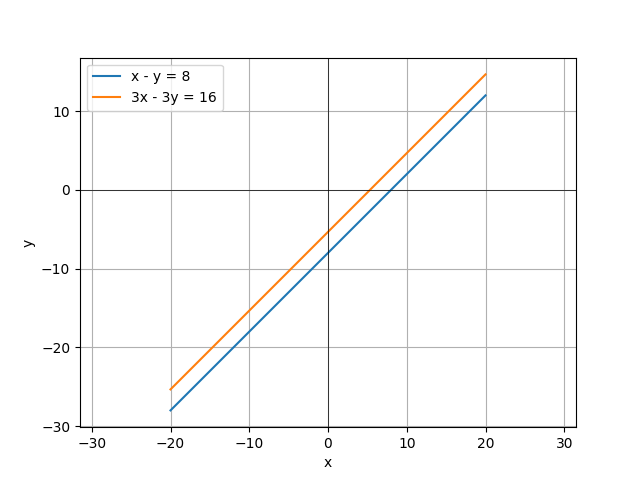
\includegraphics[width=\columnwidth]{figs/fig.png}
 \end{figure}
\end{document}

